\documentclass{article}
%% Useful packages
\usepackage[utf8]{inputenc}
\usepackage[a4paper,left=2cm,right=2cm,top=2cm,bottom=2cm]{geometry}
\usepackage{crop,graphicx,amsmath,array,color,amssymb,fancyhdr,lineno}
\usepackage{flushend,stfloats,amsthm,chngpage,times,,lipsum,lastpage} 
\usepackage{calc,listings,color,wrapfig,tabularx,longtable,enumitem}
\usepackage{amsmath}
\usepackage{biblatex} %Imports biblatex package
\usepackage[style=numeric-comp,backend=biber]
{biblatex}
\usepackage{lineno}
\usepackage{blindtext}
%%%%%%%%%%%%   Header and Footer  %%%%%%%%%%%%%
\pagestyle{fancy}
\fancypagestyle{plain}{%
  \renewcommand{\headrulewidth}{0pt}%
  \fancyhf{}%
  \page
}

\title{%
  Project Title \\
  \large Subtitle}
\author{Random Name}

\begin{document}
\begin{titlepage}

\newcommand{\HRule}{\rule{\linewidth}{0.5mm}} % Defines a new command for the horizontal lines, change thickness here

%----------------------------------------------------------------------------------------
%	LOGO SECTION
%----------------------------------------------------------------------------------------
\center
\includegraphics[width=7cm]{Title/American_International_University-Bangladesh_Monogram.png}\\[1cm] % Include a department/university logo - this will require the graphicx package
 
%----------------------------------------------------------------------------------------

\center % Center everything on the page

%----------------------------------------------------------------------------------------
%	HEADING SECTIONS
%----------------------------------------------------------------------------------------

\textsc{\LARGE \textbf{American International University-Bangladesh}}\\[1.5cm] % Name of your university/college
\textsc{\Large \textbf{Artificial Intelligence and Expert System}}\\[0.5cm] % Major heading such as course name
\textsc{\large \textbf{Section: E}}\\[0.5cm] % Minor heading such as course title
\textsc{\large  \textbf{Department of Computer Science}}\\[0.5cm] % Minor heading such as course title
\textsc{\large  \textbf{Faculty of Science and Technology}}\\[0.5cm] % Minor heading such as course title

%----------------------------------------------------------------------------------------
%	TITLE SECTION
%----------------------------------------------------------------------------------------
\makeatletter
\HRule \\[0.4cm]
{ \huge \bfseries \ Artificial Intelligence and Expert System Final Assignment}\\[0.4cm] % Title of your document
\HRule \\[1.5cm]
 
%----------------------------------------------------------------------------------------
%	AUTHOR SECTION
%----------------------------------------------------------------------------------------

\begin{minipage}{0.4\textwidth}
\begin{flushleft} \large
\emph{ \textbf{Author:}}\\
 \textbf{Fahim Mahmud Bhuiyan} % Your name
\\[1.2em]
\emph{ \textbf{ID No:}}\\
 \textbf{20-42970-1} \\[1.2em]
\end{flushleft}
\end{minipage}
~
\begin{minipage}{0.4\textwidth}
\begin{flushright} \large
\emph{ \textbf{Semester:}} \\
 \textbf{Fall 2022-23} \\[1.2em] % Supervisor's Name
\emph{ \textbf{Course Teacher:}} \\
 \textbf{Dr. Hossain Md. Shakhawat} % second marker's name 
\\ \textbf{Assistant Professor}
\end{flushright}
\end{minipage}\\[2cm]
\makeatother

% If you don't want a supervisor, uncomment the two lines below and remove the section above
%\Large \emph{Author:}\\
%John \textsc{Smith}\\[3cm] % Your name

%----------------------------------------------------------------------------------------
%	DATE SECTION
%----------------------------------------------------------------------------------------

{\large  \textbf{December 16, 2022}}\\[2cm] % Date, change the \today to a set date if you want to be precise

\vfill % Fill the rest of the page with whitespace

\end{titlepage}
\sffamily

\fancyhf{}
\fancyhead[L]{\textbf{Fahim Mahmud Bhuiyan}}
\fancyhead[R]{\textbf{Artificial Intelligence and Expert System Final Assignment}}
\fancyfoot[R]{ \bf\thepage\ \rm }%
\newpage
\tableofcontents
\pagebreak
\section{Artificial Intelligence}
\subsection{What is Artificial Intelligence?}
\large{The simulation of human intellectual functions by machines, particularly computer systems, is known as artificial intelligence. Expert systems, natural language processing, speech recognition, and machine vision are some examples of specific AI applications.}
\subsection{How does Artificial Intelligence Work?}
\large{Simply said, the way AI systems function is by combining sizable with intelligent, iterative processing algorithms. Through this combination, AI may learn from the features and patterns in the examined data. Every time an artificial intelligence system processes a cycle of data, it tests and evaluates its effectiveness and uses the data to get more knowledgeable.}
\subsection{What applications of Artificial Intelligence technology are there today?}
AI is used in many different kinds of technologies. Here are some examples:
\subsubsection{Machine learning}
The technology of getting a computer to act without programming is described here. Deep learning is a branch of machine learning that may be conceptualized as automating predictive analytics.
\subsubsection{Machine vision}
A machine now has the capacity to sight thanks to this technology. Using a camera, analog-to-digital conversion, and digital signal processing, machine vision gathers and evaluates visual data. Though frequently likened to human vision, machine vision is not constrained by biology and may be designed to, for instance, see through walls. It is utilized in a variety of applications, including medical picture analysis and signature identification. Often confused with machine vision, computer vision focuses on automated image processing.
\subsubsection{Self-driving cars}
A mix of computer vision, image recognition, and deep learning is used in autonomous cars to develop automatic ability at driving a vehicle while keeping in a set lane and avoiding unforeseen obstacles, such as pedestrians.

\begin{figure}[!htb]
    \centering
    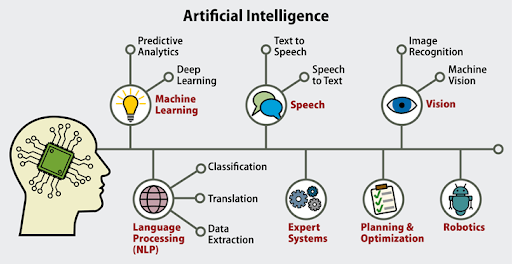
\includegraphics[width=0.6\linewidth]{ai_image.png}
    \caption{\textbf{Applications of Artificial Intelligence.}}
    \label{fig:P1Q3b}
\end{figure}

\pagebreak
\section{Forward Pass}
\subsection{What is Forward Pass?}
Forward pass is the process of computing and storing intermediate variables for a neural network from the input layer to the output layer in the correct sequence. In order to avoid circular data flow, which won't provide an output, data flows in a forward direction. The feed-forward network is a network design that facilitates forward pass.
\subsection{How does Forward Pass Work in Neural Networks?}
Step 1: Supplying the neural network with inputs. \\
Step 2: Data is obtained, processed, and then sent via an activation function through hidden layers of the network. \\
Step 3: The output is then transferred to the following layer, and so on until the last layer is reached. \\
\\\textbf{Dataset:}
\begin{center}
\begin{tabular}{||c c c c c||} 
 \hline
 Student & X1 & X2 & X3 & Y \\ [0.5ex] 
 \hline\hline
 1 & 60 & 80 & 5 & 82 \\ 
 \hline
\end{tabular}
\end{center}
\begin{figure}[!htb]
    \centering
    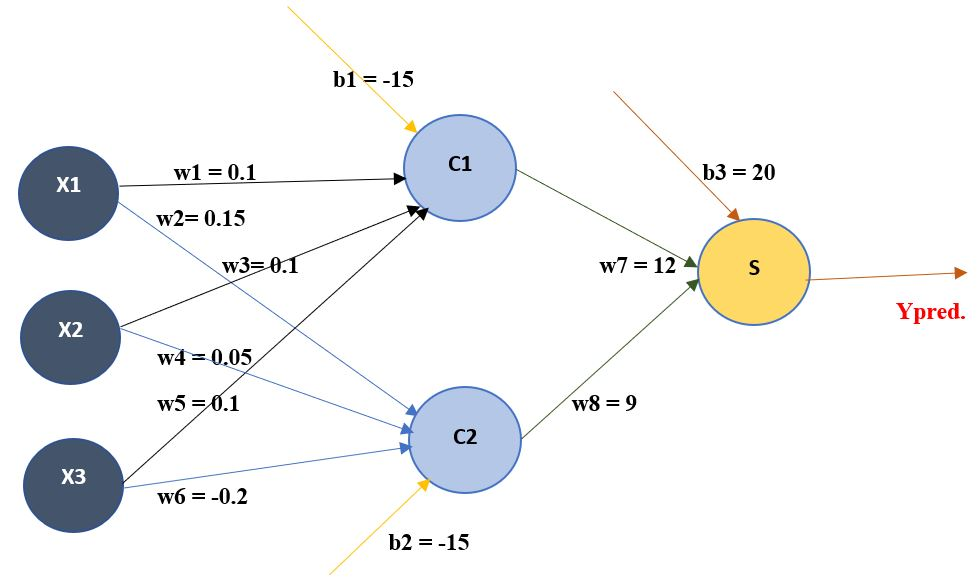
\includegraphics[width=0.85\linewidth]{Forward Pass_Examples.JPG}
    \caption{\textbf{Forward Pass in Neural Networks.}}
    \label{fig:P1Q3b}
\end{figure}
\\So, \\
\textbf{z1} = w1*X1 + w3*X2+ w5*X3 + b1 
   = 0.1*60 + 0.1*80 + 0.1*5 + (-15)
   \textbf{= -0.5}\\
\pagebreak
   \\
   Sigmoid function,
   \begin{center}
        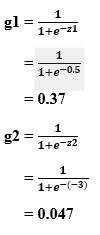
\includegraphics[width=0.25\linewidth]{Forward Pass_Equi.JPG}
   \end{center}
\textbf{z2} = w2*X1 + w4*X2+ w6*X3 + b2 = 0.15*60 + 0.05*80 + (-0.2)*5 + (-15) \textbf{= -3}
\\\textbf{Ypred.} = w7*g1 + w8*g2 + b3 = 12*0.37 + 9*0.047 + 20 \textbf{= 24.95}\\
\\ We now compare the predicted output of \textbf{24.95} with the actual output.\\
\\Doesn't look too good.
\\\textbf{24.95} is far off from \textbf{82}.\\
\\So we need a method that can update the weights so that the error between prediction and actual is reduced. This method is \textbf{Back Propagation.}\\
\pagebreak
\section{Back Propagation}
\subsection{What is Back Propagation?}
In order to train a neural network, Back Propagation is essential. It is a technique for adjusting a neural network's weights depending on the error rate recorded during the preceding epoch. By properly setting the weights, you may lower error rates and improve the generalization of the model, which will make it more dependable.\\\\
In neural networks, "backward propagation of mistakes" is referred to as "Back Propagation." It is a typical approach for educating artificial neural networks. The gradient of a loss function with respect to each weight in the network may be calculated using this approach.
\subsection{How does Back Propagation Work in Neural Networks?}
The gradient of the loss function for a single weight is calculated by the chain rule by the Back Propagation method in neural networks. It effectively computes one layer at a time, as opposed to a native direct calculation. The gradient is computed, but its application is not specified. The calculation in the delta rule is generalized by it.\\\\
Step 1: A preconnected route is used to provide inputs X.\\
Step 2: Real weights C are used to simulate the input. Typically, weights are chosen at random.\\
Step 3: Determine each neuron's output from the input layer through the hidden layers and to the output layer.\\
Step 4: Determine the output error
\begin{center}
Error of Back Propagation = Actual Output – Desired Output
\end{center}
Step 5: To change the weights such that the error is reduced, go back from the output layer to the hidden layer.\\\\
To understand, look at the following diagram of a back propagation neural network:
\begin{figure}[!htb]
    \centering
    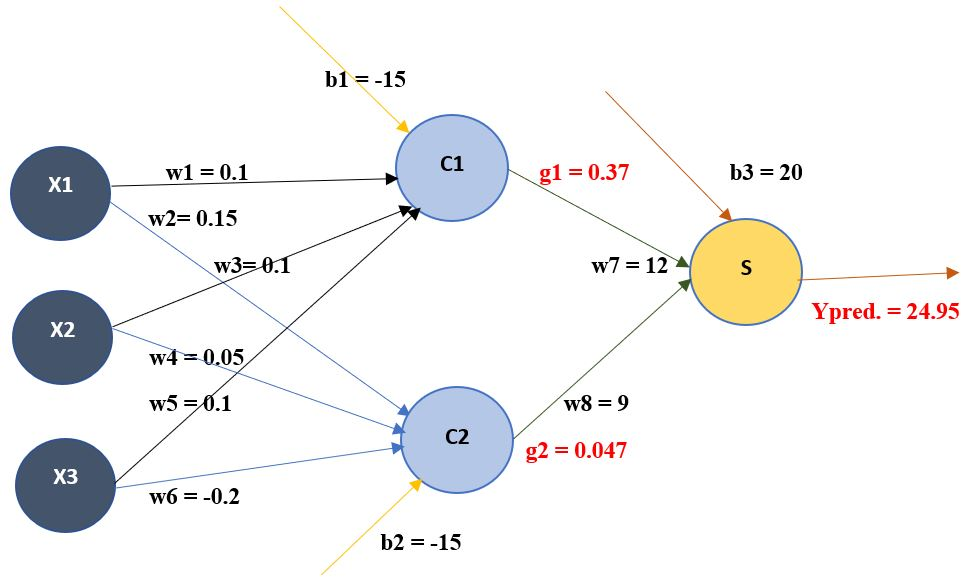
\includegraphics[width=0.85\linewidth]{Back Propagation_Examples.JPG}
    \caption{\textbf{Back Propagation in Neural Networks.}}
    \label{fig:P1Q3b}
\end{figure}
\\\textbf{Dataset:}
\begin{center}
\begin{tabular}{||c c c c c||} 
 \hline
 Student & X1 & X2 & X3 & Y \\ [0.5ex] 
 \hline\hline
 1 & 60 & 80 & 5 & 82 \\ 
 \hline
\end{tabular}
\end{center}
Partial derivative formula using the chain rule,
\begin{center}
    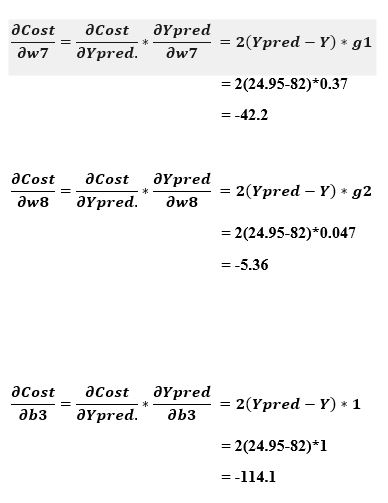
\includegraphics[width=0.45\linewidth]{Back Propagation_Partial derivative.JPG}
\end{center}
Update the weights and biases using gradient descent.\\
Walk down the cost function in the direction of the negative partial derivatives, by taking small steps, also called the learning rate.\\
\begin{center}
    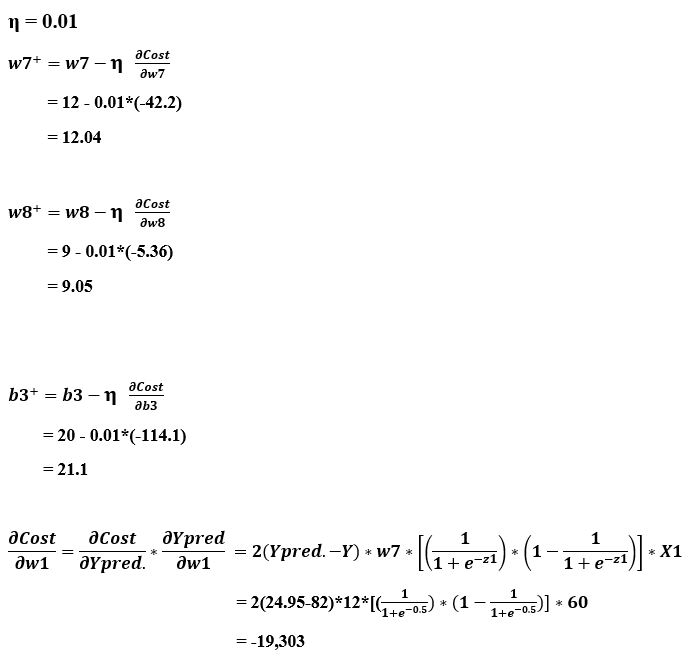
\includegraphics[width=0.66\linewidth]{Back Propagation_Equi1.JPG}\\
    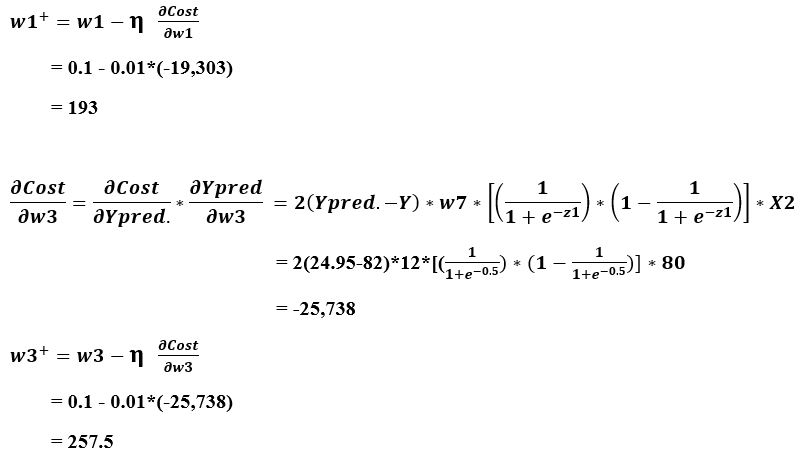
\includegraphics[width=0.85\linewidth]{Back Propagation_Equi2.JPG}\\
    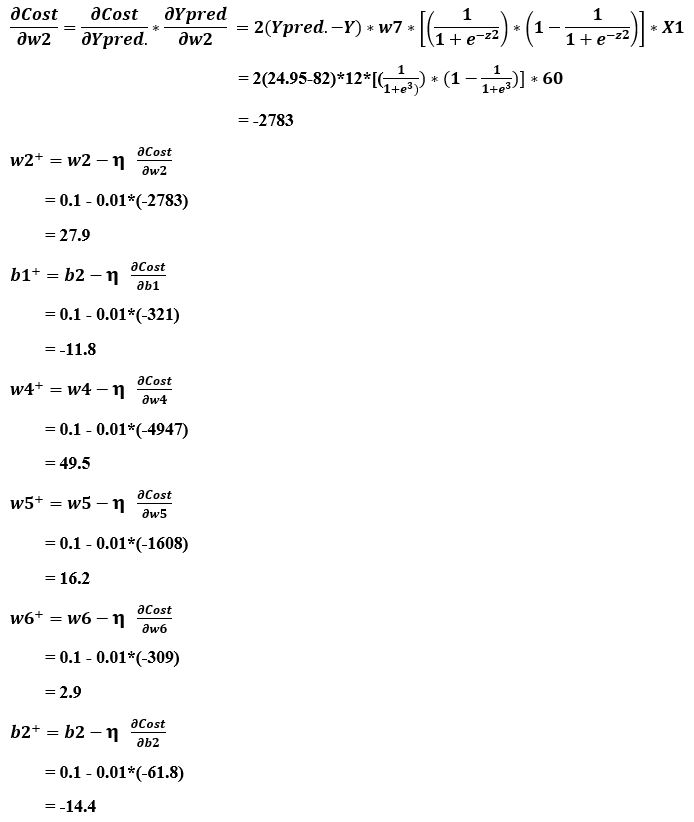
\includegraphics[width=0.85\linewidth]{Back Propagation_Equi3.JPG}
\end{center}
\pagebreak
\begin{figure}[!htb]
    \centering
    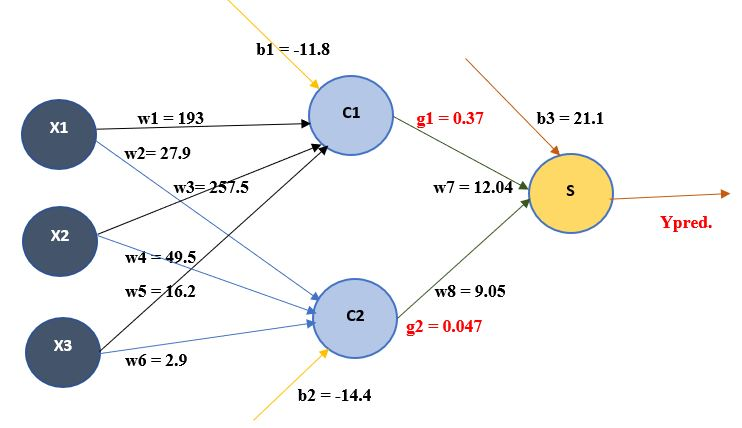
\includegraphics[width=0.85\linewidth]{Back Propagation_Updated Weights and Biases.JPG}
    \caption{\textbf{After Updated Weights and Biases, Back Propagation in Neural Networks.}}
    \label{fig:P1Q3b}
\end{figure}
\pagebreak

\bibliographystyle{amsplain}
    \begin{thebibliography}{10}
        \bibitem{beer1} Daniel Johnson, "What is Artificial Intelligence? Introduction, History & Types of AI", November 19, 2022. [Online]. Available: https://www.guru99.com/artificial-intelligence-tutorial.html
        \bibitem{beer2} Andrew Zola, "backpropagation algorithm", Aug. 2022. [Online]. Available: https://www.techtarget.com/searchenterpriseai/definition/backpropagation-algorithm
		\bibitem{beer3} Kiprono Elijah Koech, "How Does Back-Propagation Work in Neural Networks?", Jul. 09, 2022. [Online]. Available: https://towardsdatascience.com/how-does-back-propagation-work-in-neural-networks-with-worked-example-bc59dfb97f48
        \bibitem{beer4} Jeremy Jordan, "Neural networks: training with backpropagation.", Jul. 18, 2017. [Online] Available: https://www.jeremyjordan.me/neural-networks-training
        \bibitem{beer5} Rabindra Lamsal, "A step by step forward pass and backpropagation example.", Apr. 23, 2021. [Online] Available: https://theneuralblog.com/forward-pass-backpropagation-example/
    \end{thebibliography}
\end{document}